In the previous section, we have described an approach to
parameterizing models of risk group dynamics which highlights the
\textit{feasibility} of including such model components based on available data.
In this section, we explore the \textit{importance} of including these components.
The aim of these experiments is to explore the influence of
different risk group dynamics, and especially turnover, on epidemic model outputs.
To do so, we compare prevalence and incidence at equilibrium, with and without:
population growth,
heterogeneity in risk, and
risk group turnover.
We also explore the influence of different rates of turnover on
overall and group-specific equilibrium prevalence and incidence.
Finally, we highlight the importance of turnover for calibrated models,
especially when estimating the transmission population attributable fraction (TPAF)
of risk groups.
% ==================================================================================================
\subsection{Model \& Simulations}\label{ss:model-sim}
We start with a deterministic 1-sex SIR model of transmission
in a population with heterogeneity in risk.
The model is not representative of a specific infection but requires contact matching
as per a sexually transmitted infection.
The model includes three health states:
susceptible~$\mathcal{S}$, infected~$\mathcal{I}$, and recovered~$\mathcal{R}$
(Figure~\ref{fig:health-states}),
and $G = 3$ levels of risk:
high~$H$, medium~$M$, and low~$L$.
Risk levels are stratified by different rates of
contact formation across groups, reflecting sexual mixing,
so that individuals in risk group $i$ are assumed to
form contacts at a rate $C_{i}$.
The probability $\rho$ of contact formation between individuals in group $i$
with partners in risk group $k$ is assumed to
be proportionate with the total number of available contacts:
\begin{equation}
  \rho_{ik} = \frac 
    {C_k x_k}
    {\sum_{\mathrm{k}}C_{\mathrm{k}} x_{\mathrm{k}}}
    \label{eq:rho}
\end{equation}
\begin{figure}
  \centering
  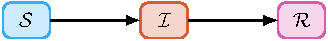
\includegraphics[width=0.4\linewidth]{health-states}
  \caption{Modelled health states.
  $\mathcal{S}$: susceptible;
  $\mathcal{I}$: infected;
  $\mathcal{R}$: recovered.}
  \label{fig:health-states}
\end{figure}
\par
Transmission of the infection from infected $\mathcal{I}$ to susceptible $\mathcal{S}$ individuals
is assumed to occur with probability $\beta$ per contact.
The force of infection for susceptible individuals in risk group $i$
is therefore modelled using the following equation:
\begin{equation}
  \lambda_{i} =
  C_{i} \sum_k \rho_{ik} \thinspace  \beta \thinspace \frac{\mathcal{I}_k}{x_k}
  \label{eq:foi}
\end{equation}
Infected individuals $\mathcal{I}$ are assumed to
be diagnosed, treated and recover at a rate $\tau$ (per year).
Recovered individuals $\mathcal{R}$ are not considered infectious,
but do not return to the susceptible state.
\par
As described in the previous section, individuals
enter the model at a rate $\nu$,
exit the model at a rate $\mu$,
and transition from risk group $i$ to group $j$ at a rate $\phi_{ij}$.
The turnover rates $\phi$ and distribution of model entrants by risk group $\bm{\hat{e}}$
are resolved using the methods outlined in
Section \ref{sss:params-turnover}. %~\nameref{sss:params-turnover}.
To this end, the following three assumptions ensure that
a unique set of $\phi$ and $\bm{\hat{e}}$ are determined
-- i.e. only one possible value for each element in $\phi$ and $\bm{\hat{e}}$
can satisfy these assumptions simultaneously.
First, the distribution of model entrants $\bm{\hat{e}}$ by risk group is assumed to equal
the distribution of individuals in the model $\bm{\hat{x}}$.
Second, it is assumed that
the average duration spent in each risk group $\bm{\delta}$ is known.
Finally, the absolute number of individuals
moving between two groups in either direction is assumed to be balanced.
The resulting system of equations which can be used to resolve $\phi$ and $\bm{\hat{e}}$
is given in \ref{aa:eqs-turnover}. %~\nameref{aa:eqs-turnover}.
\par
The above assumptions specify which parameters are defined,
but not what specific value they take.
Those parameter values are summarized for this base model in Table~\ref{tab:params-base}.
After resolving the system of equations,
$\bm{\hat{e}}$ is equal to $\bm{\hat{x}}$ (assumed),
and $\phi$ is:
\begin{equation}
\phi = \left[\begin{array}{ccc}
*      & 0.0833 & 0.0867 \\
0.0208 & *      & 0.0158 \\
0.0058 & 0.0042 & *      \\
\end{array}\right]
\end{equation}
The full system of model equations is also given in \ref{aa:eqs-model}. %~\nameref{aa:eqs-model}.
\begin{table}
  \centering
  \caption{Base model parameters.
    All rates have units $\mathrm{year}^{-1}$ and durations are in $\mathrm{years}$.}
  \label{tab:params-base}
  \begin{tabular}{clc}
	\toprule
	    Symbol     & Description                                                             &                 Value                  \\
	\midrule
	 $\bm{\beta}$  & transmission probability per contact                                    &                 $0.03$                 \\
	    $\tau$     & rate of treatment initiation among infected                             &                 $0.1$                  \\
	    $N_0$      & initial population size                                                 &                 $1000$                 \\
	\midrule
	$\bm{\hat{x}}$ & proportion of system individuals: high, medium, low activity            & $[ 0.04 \enspace 0.20 \enspace 0.76 ]$ \\
	$\bm{\hat{e}}$ & proportion of entering individuals: high, medium, low activity          & $[ 0.04 \enspace 0.20 \enspace 0.76 ]$ \\
	$\bm{\delta}$  & average duration spent in: high, medium, and low activity groups        &    $[ 5 \enspace 15 \enspace 25 ]$     \\
	     $C$       & rate of contact formation among individuals: high, medium, low activity &     $[ 25 \enspace 5 \enspace 1 ]$     \\
	    $\nu$      & rate of population entry                                                &                 $0.05$                 \\
	    $\mu$      & rate of population exit                                                 &                 $0.03$                 \\
	\bottomrule
\end{tabular}
\end{table}
\par
Epidemics are then simulated using these parameters in this model
(and variants, described below).
Each epidemic is initialized at $t = 0$ with $N_0 = 1000$ individuals,
and initial individuals distributed among risk groups according to $\bm{\hat{x}}$.
All initial individuals are susceptible $\mathcal{S}$
except for one infected person $\mathcal{I}$ in each risk group.
Each epidemic is solved numerically in Python%
\footnote{Code for all aspects of the project is available at:
  \href{https://github.com/c-uhs/turnover}{\texttt{https://github.com/c-uhs/turnover}}}
using Euler's method with a time step of $dt = 0.1$ years.
The model is assumed to be at equilibrium after $t = 500$ years,
which was verified qualitatively. % JK: another way of saying this?
% ==================================================================================================
\subsection{Model Variants}\label{ss:exp-variants}
Consider the risk group dynamics outlined in Box~\ref{box:assumptions}.
The assumption b) in each case is taken to be generally more plausible:
populations \textit{are} heterogeneous in risk;
turnover among risk groups \textit{does} occur; and
population growth \textit{does} occur.
These assumptions are reflected in the base model, described above.
However, many epidemic models do not make these assumptions.
The following experiments aim the illustrate the potential influence
of such assumptions on model outputs.
In each case, a model variant is constructed
which makes the alternate assumption a):
1.1) populations \textit{are not} heterogeneous in risk;
1.2) turnover among risk groups \textit{does not} occur; and
1.3) population growth \textit{does not} occur.
An epidemic is then simulated with fixed parameter values
using both the base model and the variant.
Overall projected incidence and prevalence are then compared between the models.
The details of each model variant are summarized as follows.
% --------------------------------------------------------------------------------------------------
\paragraph{Experiment 1.1: Risk Heterogeneity}\label{p:exp-1-hetero}
The first variant (V1) is defined
to no longer consider heterogeneity in risk.
The three risk groups are combined,
and the new contact rate $C$ for all individuals is defined as
the weighted average of previously risk-stratified $C_i$.
It is also no longer possible to include turnover,
as there is only one risk group.
The number of individuals who are initially infected remains as three.
% No other parameters are changed as no other parameters
% were originally stratified by risk.
% --------------------------------------------------------------------------------------------------
\paragraph{Experiment 1.2: Population Growth}\label{p:exp-1-growth}
Another variant (V2) is defined which does not model population growth.
In this case, the exit rate $\mu$ remains fixed
but the entry rate $\nu$ is reduced to equal $\mu$.
This ensures that the average duration of individuals in the model $\mu^{-1}$ remains unchanged.
% --------------------------------------------------------------------------------------------------
\paragraph{Experiment 1.3: Turnover}\label{p:exp-1-turnover}
Finally, variant (V3) is defined with all turnover rates $\phi = 0$.
Following Eq.~(\ref{eq:duration-group}),
this is equivalent to assuming that the duration in each group is equal to
the average duration of individuals in the model $\mu^{-1}$.
Since the distribution of risk behaviour in the entering population $\bm{\hat{e}}$
was assumed to be equal to that in the model $\bm{\hat{x}}$,
no other modifications are required.
\par
The model variants constructed for each experiment
are summarized in Figure~\ref{fig:variant-tree},
and the corresponding parameters are given in Table~\ref{tab:params-variants}.
\begin{figure}
  \centering
  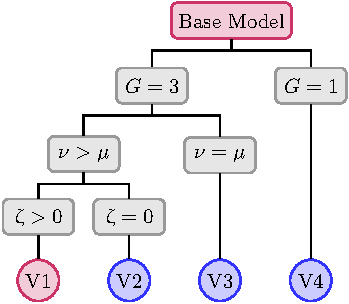
\includegraphics[width=0.7\linewidth]{variant-tree}
  \caption{Summary of four model variants
    with respect to simulated risk group dynamics.
    Relative risk group size is the same in all variants.
    $G$:~number of risk groups,
    $\nu$:~rate of population entry,
    $\mu$:~rate of population exit,
    $\phi$:~rates of population turnover.}
  \label{fig:variant-tree}
\end{figure}
\begin{table}
  \centering
  \caption{Parameters for model variants.
    All rates have units $\mathrm{year}^{-1}$ and durations are in $\mathrm{years}$.
    Vectors correspond to parameters stratified by high, medium, and low risk groups.}
  \label{tab:params-variants}
  \begin{threeparttable}
\begin{tabularx}{0.95\linewidth}{c *{4}{Y}}
	\toprule
	  Parameter    & Full                     & V1                           & V2                       & V3                                         \\
	\midrule
	$\bm{\hat{x}}$ & $[ 0.05\es0.20\es0.75 ]$ & ---                          & $[ 0.05\es0.20\es0.75 ]$ & $[ 0.05\es0.20\es0.75 ]$                   \\
	$\bm{\hat{e}}$ & $[ 0.05\es0.20\es0.75 ]$ & ---                          & $[ 0.05\es0.20\es0.75 ]$ & $[ 0.05\es0.20\es0.75 ]$                   \\
	     $C$       & $[ 25\es5\es1 ]$         & $[ \textbf{3} ]$\tnote{a}    & $[ 25\es5\es1 ]$         & $[ 25\es5\es1 ]$                           \\
	   $\delta$    & $[ 5\es15\es25 ]$        & $[ \textbf{33.3} ]$\tnote{b} & $[ 5\es15\es25 ]$        & $[ \textbf{33.3\es33.3\es33.3} ]$\tnote{b} \\
	    $\nu$      & $0.05$                   & $0.05$                       & $\textbf{0.03}$\tnote{c} & $0.05$                                     \\
	    $\mu$      & $0.03$                   & $0.03$                       & $0.03$                   & $0.03$                                     \\
	\bottomrule
\end{tabularx}
\footnotesize
\begin{tablenotes}
  \item
  $\bm{\hat{x}}$: proportion of individuals in the model by risk group (high, medium, low);
  $\bm{\hat{e}}$: proportion of individuals entering the model by risk group;
  $C$: rate of contact formation by risk group (per year);
  $\delta$: average duration in each risk group (years);
  $\nu$: rate of population entry (per year);
  $\mu$: rate of exit (per year).
  \item[a] Weighted average of risk-stratified $C$
  \item[b] Without turnover, duration in all groups must be equal to the inverse of the exit rate, $\mu^{-1}$
  \item[c] Adjusting the entry rate, versus exit rate, does not affect average duration in the model
\end{tablenotes}
\end{threeparttable}
\end{table}
% ==================================================================================================
\subsection{Influence of Turnover}\label{ss:exp-turnover}
As noted above, the influence of turnover on equilibrium prevalence and incidence
depends on several factors, including
turnover magnitude and duration of infectiousness.
To help understand trends in model outputs with respect to these factors,
the base model is used to explore
a range of turnover magnitudes and durations of infectiousness.
% --------------------------------------------------------------------------------------------------
\paragraph{Experiment 2.1: Turnover Magnitude}
First, the magnitude of turnover is considered alone,
for fixed duration of infectiousness.
As in similar experiments \citep{Zhang2012,Henry2015},
the rates of turnover are scaled by a single parameter.
However, since the model used here has $G = 3$ risk groups,
it is not possible to simply multiply a set of base rates $\phi$ by a scalar factor;
this would result in changes to the equilibrium risk group sizes,
which is avoided throughout this work.
Rather, the rates of turnover are controlled by
the duration of individuals in the high risk group $\delta_H$ in the following way.
The distribution of model entrants $\bm{\hat{e}}$ is again assumed to equal
the distribution of individuals in the model $\bm{\hat{x}}$.
The absolute number of individuals moving between two groups in either direction
is also assumed to be balanced, as before.
% Then, the duration of individuals in the high risk group $\delta_H$
% is used as the controlling parameter.
The duration of individuals in the medium risk group $\delta_M$
is then defined as a value between $\delta_H$ and the maximum duration $\mu^{-1}$
which scales with $\delta_H$ following the equation:
$\delta_M = \delta_H + \kappa \left(\mu^{-1} - \delta_H\right)$, with $\kappa = 0.3$.
Finally, the duration of individuals in the low risk group $\delta_L$
similarly scales with $\delta_H$,
but the value is not required to resolve $\phi$;
it can be determined from $\phi$ afterwards
using Eq.~(\ref{eq:duration-group}).
In this way, each value of $\delta_H$ can be used to compute a set of turnover rates $\phi$
whose elements all scale inversely with the duration in the high risk group $\delta_H$.
The value of $\delta_H$ is then varied from 3~to~33 years,
and trends in the equilibrium incidence and prevalence are plotted
for each group, as well as overall.
%The duration in a risk group is also perhaps easier to grasp
%than individual transition rates.
%\footnote{Throughout this work,
%  we define duration $\delta_i$ as a ``single average pass through the group''
%  which does not consider reentrance after exiting to another group.}
% JK: I feel like these limits need justification,
% but its difficult to give without grounding in any specific infections
\par
% --------------------------------------------------------------------------------------------------
\paragraph{Experiment 2.2: Turnover and Treatment Rate}
Next, the above experiment is repeated for a range of treatment rates.
The treatment rate controls the duration of infectiousness $\delta_{\mathcal{I}}$
as in $\delta_{\mathcal{I}} = \tau^{-1}$.
Treatment rate $\tau$ is varied from 1~to~0.05,
implying a duration of infectiousness of 1~to~20 years.
The duration in the high risk group $\delta_H$ is varied from 3~to~33 years as before,
and trends equilibrium incidence and prevalence are again shown,
this time using 2D surface plots.
% ==================================================================================================
\subsection{Implications for Model Fitting}\label{ss:exp-turnover-fit}
Finally, since almost all context-specific applications of epidemic models entail
fitting uncertain model parameters to data-driven calibration targets,
some potential implications of omitting turnover from a fitted model are explored.
In particular, the influence of turnover on two model outputs are estimated,
before and after model fitting:
the inferred level of risk heterogeneity in the population;
and the transmission population attributable fraction (TPAF)~\citep{Mishra2016}
of the high risk group.
TPAF estimates the proportion of cumulative new infections which are attributable to
prevention gaps among a specific population.%
\footnote{To estimate TPAF of the high risk group,
  transmission ``from'' the high risk group is turned off, not ``to''.}
% --------------------------------------------------------------------------------------------------
\paragraph{Experiment 3.1: Inferred Risk Heterogeneity}
First, the Base model (turnover) and model variant V3 (no~turnover) are both calibrated to
25\% prevalence in the high risk group, and
5\% prevalence in the low risk group at equilibrium.
The fitted parameters are
the contact rates of the high and low risk groups: $C_H$~and~$C_L$.%
\footnote{The fitted parameters are estimated by minimizing
  the negative log-likelihood of each predicted prevalence versus the target
  (assuming a sample size of 1000)
  using the Sequential Least SQuares Programming (SLSQP) method~\citep{Kraft1988}
  from the \texttt{scipy.optimize.minimize} Python package.}
The ratio of fitted contact rates $C_H~/~C_L$
represents the degree of risk heterogeneity in the population
which must be present in order to observe the given prevalence ratio.
Comparing the fitted contact rates with and without turnover,
the influence of turnover on inferred risk heterogeneity is shown.
% --------------------------------------------------------------------------------------------------
\paragraph{Experiment 3.2: TPAF of the High Risk Group}
The level of risk heterogeneity has presumed implications
for prioritization of risk groups for interventions.
The TPAF of a risk group provides an estimate of
the importance of prioritizing the group.
Thus, differences in inferred risk heterogeneity due to turnover from Experiment 3.1
are hypothesized to result in differences in the estimated TPAF of the high risk group.
To test this hypothesis, the TPAF of the high risk group
is calculated and compared across the model variants with and without turnover,
before and after fitting to group-specific prevalence, as described above.